\documentclass{article}
\usepackage[spanish]{babel}
\usepackage[utf8]{inputenc}
\usepackage[top=20mm, bottom=20mm, left=15mm, right=15mm]{geometry}
\usepackage{amsmath}
\usepackage{graphicx}
\usepackage{float}
\usepackage{listings}
\usepackage{color}
\usepackage[all]{xy}
\definecolor{codeblue}{RGB}{0,128,255}
\definecolor{codegray}{rgb}{0.5,0.5,0.5}
\definecolor{codepurple}{rgb}{0.58,0,0.82}
\definecolor{pink}{RGB}{255,26,117}
\definecolor{backcolour}{rgb}{1,1,1}
    
\lstdefinestyle{mystyle}{
    backgroundcolor=\color{backcolour},
    commentstyle=\color{codeblue},
    keywordstyle=\color{pink},
    numberstyle=\tiny\color{codeblue},
    stringstyle=\color{codepurple},
    basicstyle=\footnotesize,
    breakatwhitespace=false,         
    breaklines=true,                 
    captionpos=b,                    
    keepspaces=true,                 
    numbers=left,                    
    numbersep=7pt,                  
    showspaces=false,                
    showstringspaces=false,
    showtabs=false,                  
    tabsize=2,
    frame=tb
}

\lstset{style=mystyle}

\title{
    Reconocimiento de letras manuscritas con redes neuronales artificiales\\ 
    \large Tercera y cuarta entrega}
\author{Edson Raul Cepeda Marquez \\ Sonia Alejandra Treviño Rivera}
\date{\today}

\begin{document}
\setlength{\parskip}{2mm}
\setlength{\parindent}{0pt}
\maketitle
\section{Resumen}\label{sec:Resumen}
Este proyecto consiste en una aplicación web que implementa una red neuronal artificial capaz 
de reconocer letras manuscritas. La aplicación web en cuestión está desarrollada con tres tecnologías 
que se conectan y permiten su uso:
\begin{enumerate}
    \item \textbf{Angular}: Un framework de código libre desarollado por Google que facilita el desarrollo de 
    aplicaciones web de una sola página (SPA: Single Page Applicaction). Tiene la ventaja de separar completamente el frontend y el backend lo que permite
    seguir facilmente el patrón de diseño MVC (Modelo-Vista-Controlador). 
    \item \textbf{Express}: Un framework de desarrollo web que utiliza el entorno de ejecución Node JS y facilita la creación de REST APIs.
    \item \textbf{Python}: Un lenguaje de programación interpretado orientado a objetos. Tiene la ventaja de ser simple, lo que permite escibir código legible.
    Tiene una amplia comunidad de desarrollo y una gran cantidad de librerias para todo tipo de tareas.
\end{enumerate}
En la figura \ref{flujo} se muestra un diagrama que representa el flujo de información entre las tres tecnologías. Se puede observar que la información fluye en ambas direcciones. 
\begin{figure}[H]
    \begin{displaymath}
        \xymatrix{*+<1cm>[F]{Angular} \ar[r] & *+<1cm>[F]{Express} \ar[l] \ar[r] & *+<1cm>[F]{Python} \ar[l]}
    \end{displaymath}
    \caption{Flujo de información de la aplicación.}
    \label{flujo} 
\end{figure}

La aplicación web además de contener este proyecto, tiene otras secciones asignadas para proyectos futuros. Para este proyecto la sección importante es ``Imchar''. 
Esta sección de la aplicación web contiene una cuadricula con la que se puede interactuar a traves del ratón. 
\begin{figure}[H]
    \centering
    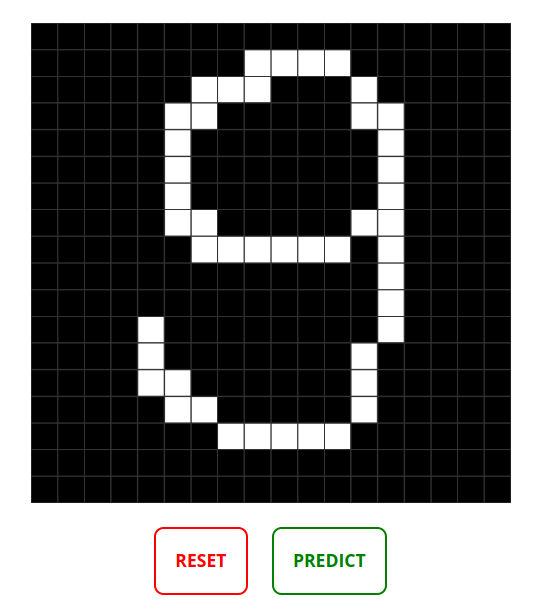
\includegraphics[width=40mm]{grid2.png}
    \caption{Cuadricula de la aplicación.}
    \label{grid}
\end{figure}
Esta es la puerta para el uso de la red neuronal artificial. 
En esta cuadricula es posible dibujar letras.
\\ Al dibujar una letra en la cuadricula y presionar el botón de ``Predeict'' la aplicación web realiza una petición al servidor de la REST API de express,
la cual recibe el estado de la cuadricula y sus dimensiones. \\
Posteriormente el servidor de express ejecuta un proceso asincrono de python el cual ejecuta un script que lleva a cabo una transformación de los datos enviados en la petición  \\
Por ultimo los datos transformados de la cuadricula son procesados por la red neuronal previamente entrenada, y devuelve una respuesta al frontend convertida en el caracter que la red neuronal predice (Figura \ref{response}).
\begin{figure}[H]
    \centering
    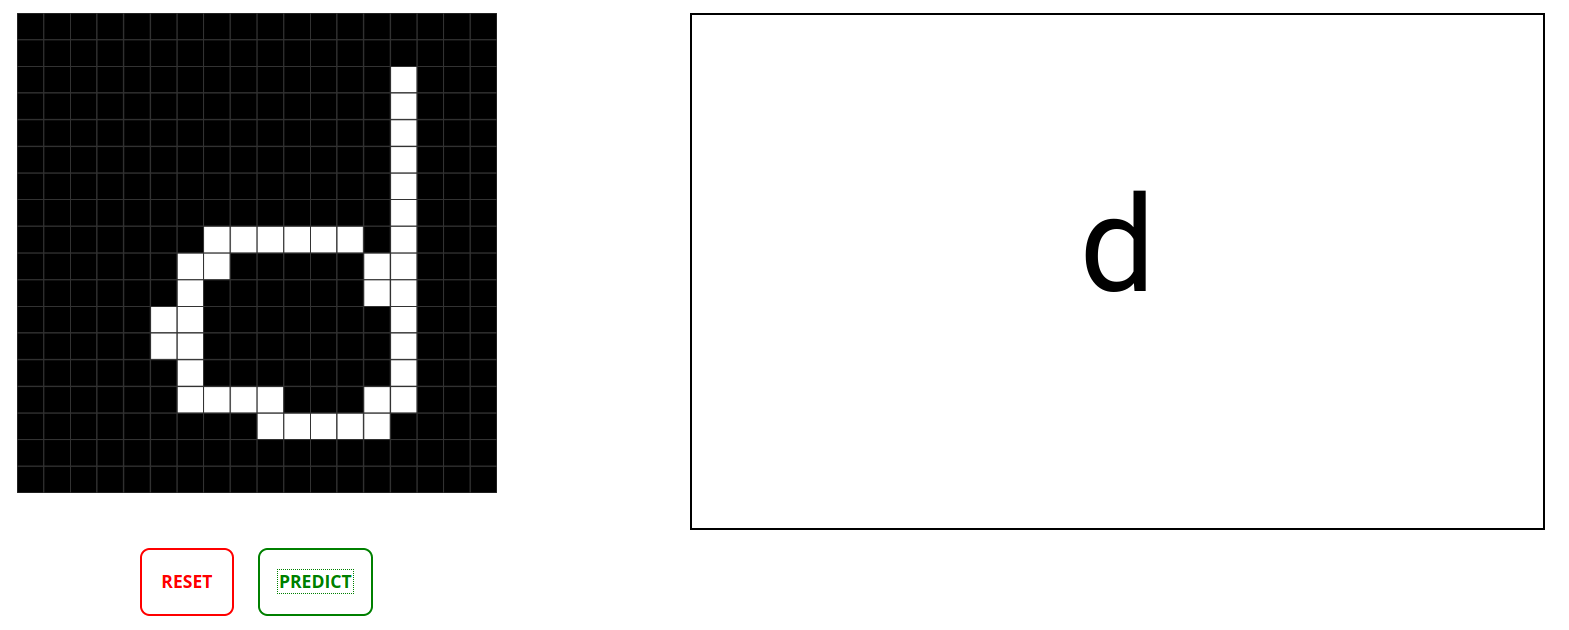
\includegraphics[width=180mm]{response.png}
    \caption{Respuesta de la red neuronal, también incluye el botón ``Reset'' para borrar la cuadricula.}
    \label{response}
\end{figure}
\textbf{Para el desarrollo de la red neuronal artificial no se utilizo ninguna librería, todo código correspondiente al algoritmo de aprendizaje fue escrito desde cero.} \\
Así mismo la red neuronal que procesa la información fue entrenada con un conjunto de datos creado desde cero, para esto se implemento una ruta oculta (figura \ref{trainer}) en la aplicación web en la que es posible utilizar la cuadricula para generar 
un conjunto de entranamiento.
\begin{figure}[H]
    \centering
    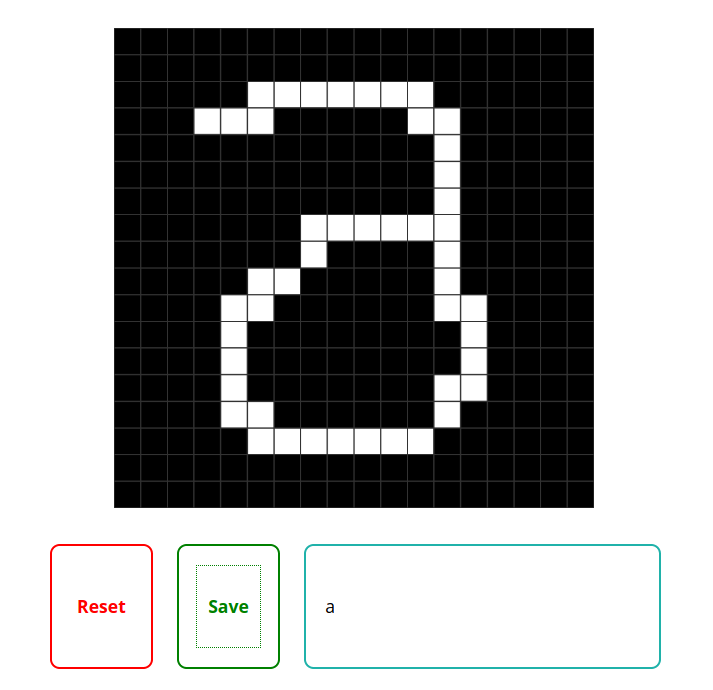
\includegraphics[width=60mm]{trainer.png}
    \caption{Ruta oculta para la generación de datos de entrenamiento}
    \label{trainer}
\end{figure}
Los resultados de entrenar la red neuronal con estos datos son que, para las 26 letras del abecedario en ingles por lo menos 21 son predichas correctamente. Las letras que presentan más problemas para ser predichas correctamente son aquellas que 
comparten cierta similaridad. La red neuronal fue entrenada multiples veces para poder llegar a una configuración de hiperparametros con un mejor rendimiento. 

\section{Introducción}\label{sec:Introduccion}
El problema que se intenta resolver al diseñar este sistema, es el de reconocer texto manuscrito para su digitalización. 
Se diseña una red neuronal convolucional que es entrenada con un conjunto de datos que contiene pequeñas imagenes de letras del abecedario en ingles. 
En la sección \ref{sec:Resumen} de este documento, se indica en que consiste el proyecto.  \\
La teoría necesaria para la realización de este proyecto se encuentra en la sección \ref{sec:Marco} \\
En la sección \ref{sec:Desarrollo} se revisa la implementación a detalle del sistema al igual que el diseño de la red neuronal. 
Por utlimo en la sección \ref{sec:Conclusion} se incluye una conclusión de lo que fue el proyecto incluyendo una introspección del equipo y trabajo a futuro. 
Todas la referencias utilizadas para este proyecto se incluyen en la sección de referencias.

\section{Marco teórico}\label{sec:Marco}
Una red neuronal artificial es un modelo matemático y un algoritmo de aprendizage automático inpirado en el funcionamiento de las neuronas biologicas que se encuentran en el cerebro.
El elemento básico de una red neuronal es la neurona. Una neurona se compone de cuatro partes fundamentales:
\begin{enumerate}
    \item \textbf{Dendrita}: Son ramificaciónes que conectan con el el cuerpo celular de una neurona, es la parte encargada de transportar los impulsos electricos.  
    \item \textbf{Cuerpo celular}: Es la parte de la neurona encargada de procesar la suma de los impulsos electricos recibidos de las dentritas. Posteriormente, se decide si disparara otra señal electrica de salida por el axon mediante un umbral.
    \item \textbf{Axon}: Son las ramificaciones finales de la neurona, transportan el impulso de salida de la neurona tras haber sido procesado en el cuerpo celular.
    \item \textbf{Sinapsis}: El punto de contacto entre el axon de una neurona y la dendrita de otra neurona. 
\end{enumerate} 
Es la organización de las neuronas y la fuerza de las sinapsis lo que establece la función principal de una neurona. En la figura \ref{neuron} se puede observar cada una de las partes de la neurona. 
\begin{figure}[H]
    \centering
    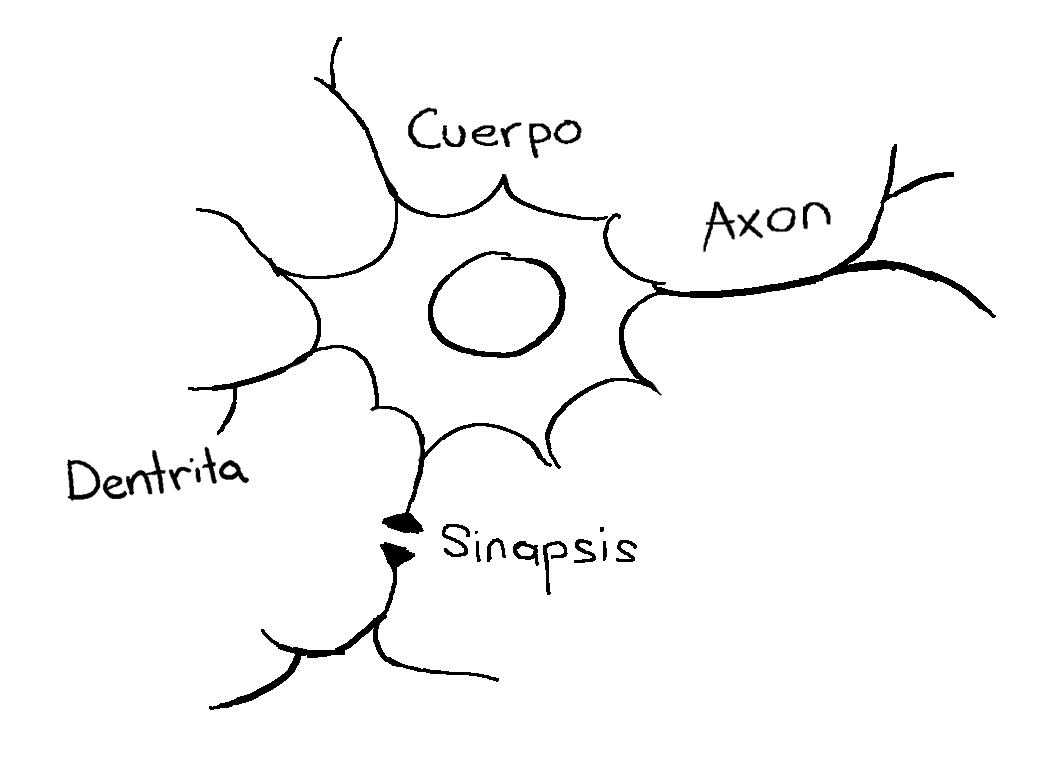
\includegraphics[width=130mm]{neuron.png}
    \caption{Neurona biologica}
    \label{neuron}
\end{figure}
Con esto es posible construir un modelo matemático de una neurona artificial (figura \ref{modelo}). En este modelo se tiene un escalar $p$ que corresponde a la señal del impulso electrico recibido de otras neuronas, $p$ es multiplicado por $w$ que corresponde a la fuerza de la sinapsis. 
Este producto $wp$ es enviado a una sumatoria y se incluye una entrada de sesgo $b$ con un valor de 1. La salida de la sumatoria $n$ va a una función de activación $f$ lo cual produce un escalar de salida $a$.
\begin{figure}[H]
    \centering
    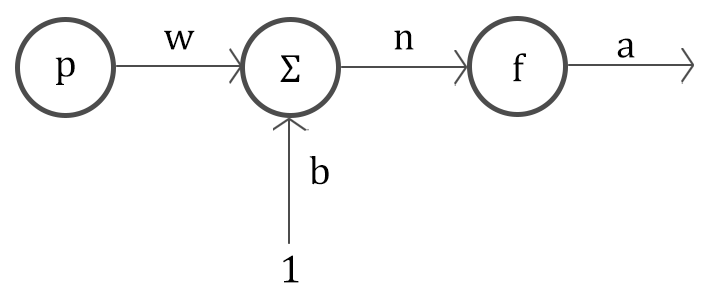
\includegraphics[width=85mm]{model.png}
    \caption{Modelo matemático de neurona artificial.}
    \label{modelo}
\end{figure}
De esta manera la salida de la neurona es calculada de la forma $a = f(wp + b)$. \\
La organización de multiples capas y multiples neuronas es lo que le da el poder a este algoritmo. A esto se le conoce como \textbf{red neuronal profunda}. 
Una red neuronal es también conocida como un aproximador de funciones universal, puesto es capaz de aproximar cualquier función teniendo la configuración adecuada.\\
El modelo matematico de una capa de una red neuronal profunda es, un vector \textbf{p} de tamaño $R$ como entrada,un determinado número de neuronas $S$, seguido de una matriz de pesos \textbf{W} con un tamaño $S\times$$R$ y un vector \textbf{b} de sesgo de tamaño $S\times1$. 
La operación \textbf{Wp + b} es enviada a una sumatoria que resulta en un vector de resultados \textbf{n} de tamaño $S\times1$ y que se dirige a una función de activación $f$ que da una vector \textbf{a} de tamaño $S\times1$ como salida. La salida de una capa es la entrada de la otra.
Para definir la arquitectura de una red neuronal se necesita definir una serie de parametros:
\begin{enumerate}
    \item Número de capas
    \item Número de neuronas por capa
    \item Tasa de aprendizage
    \item Funciones de activación de las neuronas
    \item Función de error de la red
\end{enumerate}
A estos se les conoce como \textbf{hiperparametros de la red}. Una red neuronal profunda (figura \ref{multi}) recibe su nombre del hecho que tiene una cantidad considerable de capas intermedias llamadas \textbf{capas ocultas}.
\begin{figure}[H]
    \centering
    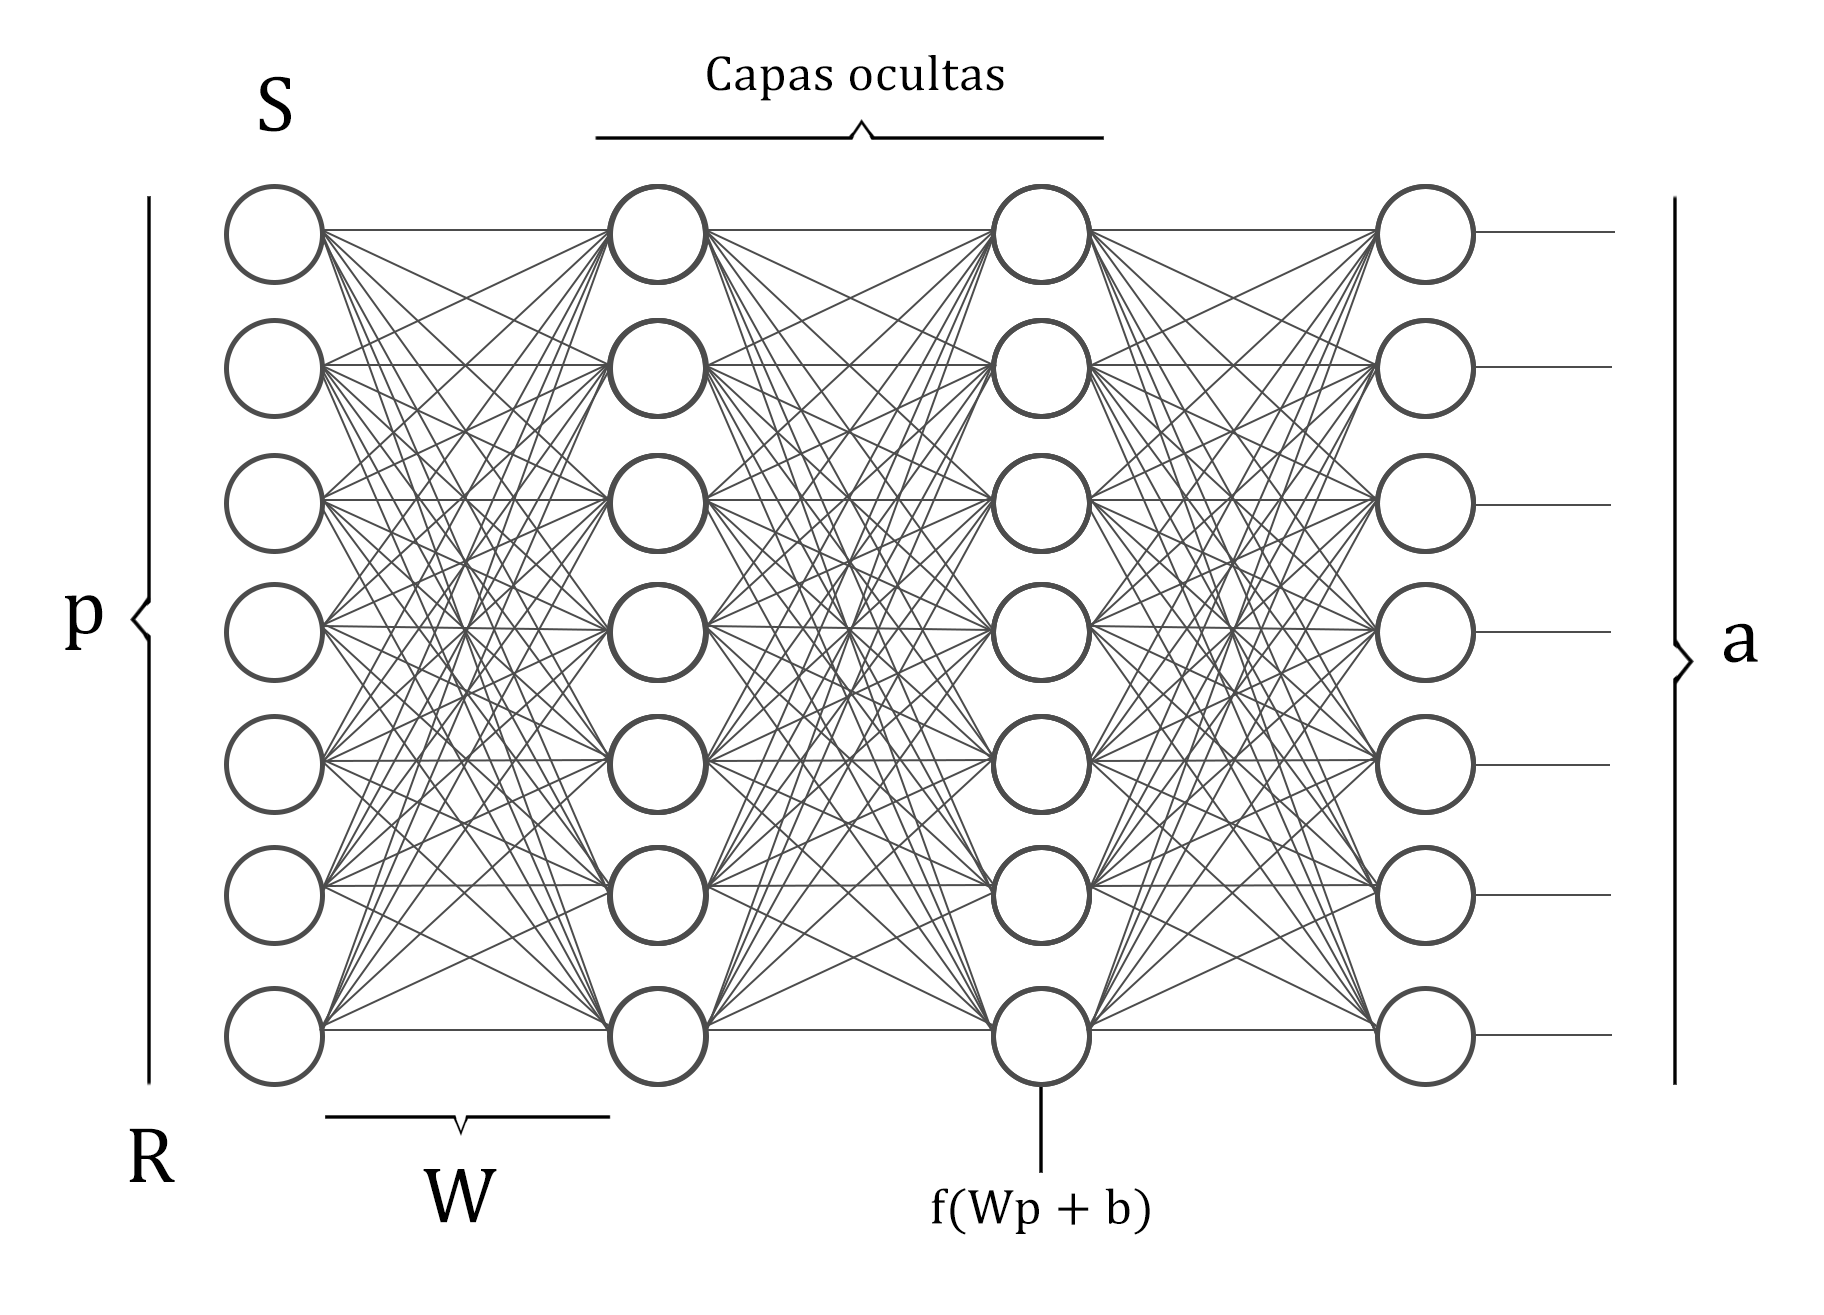
\includegraphics[width=100mm]{multi.png}
    \caption{Diagrama representativo de una red neuronal profunda}
    \label{multi}
\end{figure}
Al definir el número de neuronas de una capa también se tiene que escoger una función de activación adecuada.
Existen distintas funciones de activación que son comúnmente usadas en las redes neuronales. Las tres más comúnes son las siguientes:  \\
\textbf{Función sigmoidal o logistica}: Esta función se encuentra en el rango de 0 a 1. Es muy útil para modelos que requieren predecir una probabilidad. 
\begin{equation}
    f(x) = \frac{1}{1 + \exp^-x}
\end{equation}
\textbf{Función tangente hiperbolica}: Tambíen es una función logistica pero mejorada, el rango de esta función esta entre -1 a 1. Las ventajas de usar esta función es que penaliza fuertemente las entradas negativas. Es comúnmente usada para la clasificación de dos clases. 
\begin{equation}
    f(x) = \frac{1 - \exp^-2x}{1 + \exp^-2x}
\end{equation}
\textbf{ReLU (Unidad lineal rectificadora)}: Esta función es la más usada en las capas ocultas de las redes profundas puesto que evita el problema del desvanecimiento del gradiente que presentan las dos funciones anteriores. Esta función tiene un rango de 0 a infinito. 
Las entradas iguales o menores a cero se hacen cero, por lo que en algunos casos esto impide que se aprenda bien de los datos. Existen modificaciones de esta función que pretenden arreglar este problema como \textbf{Leaky ReLU} o \textbf{Randomized ReLU}. 
\begin{equation}
    f(x) = 
    \begin{cases}
        0, & x < 0 \\
        x, & x >= 0
    \end{cases}
\end{equation}
Las tres funciones anteriores son facílmente diferenciables lo que las hace adecuadas para el algoritmo de aprendizaje. El algoritmo más utilizado es el de propagación hacía atras o mejor conocido en ingles como \textbf{Backpropagation}. \\
Backpropagation es un algoritmo de aprendizaje que tiene como objetivo minimizar una función de error mediante el uso del \textbf{descenso del gradiente}. 
El entrenamiento de una red neuronal con este algoritmo consta de tres etapas:
\begin{enumerate}
    \item \textbf{Feedfoward}: Esta etapa consiste en propagar las entradas hacia delante en la red para obtener un resultado, este resultado se compara con el resultado esperado de la entrada y se calcula un error. 
    \item \textbf{Backpropagation}: Esta etapa consiste en calcular cuanto cambia el error si se ajustan cada uno de los pesos de la red neuronal. Se calcula una sensibilidad para los pesos derivando parcialmente la función de error respecto a cada peso. 
    \item \textbf{Actualización de pesos}: Usando las sensibilides calculadas en la etapa anterior se realiza una actualización en los valores de los pesos. 
\end{enumerate}
Este procedimiento es repetido multiples veces y con distintas entradas, estas son las \textbf{iteraciones} del entrenamiento. De esta manera la red es alimentada con suficientes ejemplos como para generalizar correctamente y reducir el error lo mejor posible.
Existen distintas architecturas que resuelven distintos tipos de problemas. Dos de las más comunes son:
\begin{enumerate}
    \item \textbf{Red neuronal convolucional}: es usada comúnmente para la clasificación de imagenes. Esta red neuronal consta de una serie de capas de extracción de caracteristicas que utiliza tecnicas de visión computacional. Las salidas de estas capas son conectadas con una serie de capas finales densas (totalmente conectadas) en las que se lleva a cabo el aprendizage.
    \item \textbf{Red neuronal recurrente}: es usada ampliamente en el campo de \textbf{procesamiento de lenguaje natural}, estas redes neuronal reciben su nombre debido a que existe una retroalimentación entre las capas.
\end{enumerate} 
Las redes neuronales como algoritmos de aprendizage automatico supervisado, realizan el proceso de aprendizage con conjuntos de datos previamente etiquetados. La calidad de este conjunto de datos refleja la calida de las predicciones de una red neuronal. \\
Otro de los factores que influyen en el rendimiento de la red neuronal, es la configuración de los hiperparametros. Existen problemas que requieren más o menos neuronas, otros que requieren más capas o menos capas. Es por esto que los hiperparametros de una red neuronal también pueden ser configurados automaticamente con el uso de otros algoritmos tales como \textbf{el algoritmo genetico}.




\section{Desarrollo}\label{sec:Desarrollo}
\section{Conclusion}\label{sec:Conclusion}

\end{document}El flujo de información entre las tres herramientas 
